\documentclass{beamer}
%\documentclass[handout]{beamer}

\usetheme{Copenhagen}
\usecolortheme{seahorse}


% for handouts, use with
% \documentclass[handout]{beamer}
%\usepackage{pgfpages}
%\pgfpagesuselayout{4 on 1}[a4paper, border shrink=5mm]


% hide navigation butons at bottom
\setbeamertemplate{navigation symbols}{}

%hide navigation at top
\setbeamertemplate{headline}{}

\setbeamercovered{transparent}


\usepackage[ngerman]{babel}
\babelprovide[hyphenrules=ngerman-x-latest]{ngerman}

\usepackage{csquotes}
\usepackage[backend=biber]{biblatex}
\addbibresource{../Ausarbeitung/Proseminar.bib}

\usepackage{graphicx}
\usepackage{tikz}

\title{Übertragung von Signalen auf elektrischen Leitungen}
\author{Sven Schmidt}


\begin{document}

% Title page with image at the top
\begin{frame}
    \centering
    % Insert and center the image at the top
    
\includegraphics[width=0.5\textwidth]{logo_fernuni_hagen.png}
    \vspace{0.5cm} % Adjust space between image and title as needed

    {\LARGE \textbf{\inserttitle}}\\[0.5cm]

    \textbf{Proseminar Mathematik in der Technik}\\
    \textbf{Modulnummer:} 61711\\
    Fakultät für Mathematik + Informatik\\[0.5cm]

    \begin{tabbing}
        \hspace{4cm} \= \kill
        \textbf{Name:} \> Sven Schmidt \\
        \textbf{Matrikelnummer:} \> 4125169 \\
        \textbf{Prüfer:} \> PD Dr.-Ing. Stefan Helfert \\
    \end{tabbing}

    \vfill

    {\large FernUniversität in Hagen}\\
    {\large Sommersemester 2025}
\end{frame}

\begin{frame}{Inhalt}
    \tableofcontents
\end{frame}

\section{Herleitung der Telegraphenleitung}


\begin{frame}{Modell des Zweidrahtleiters}

Wir betrachten ausschließlich Paralleldrahtleiter.

\begin{figure}[!htb]
    \begin{center}
        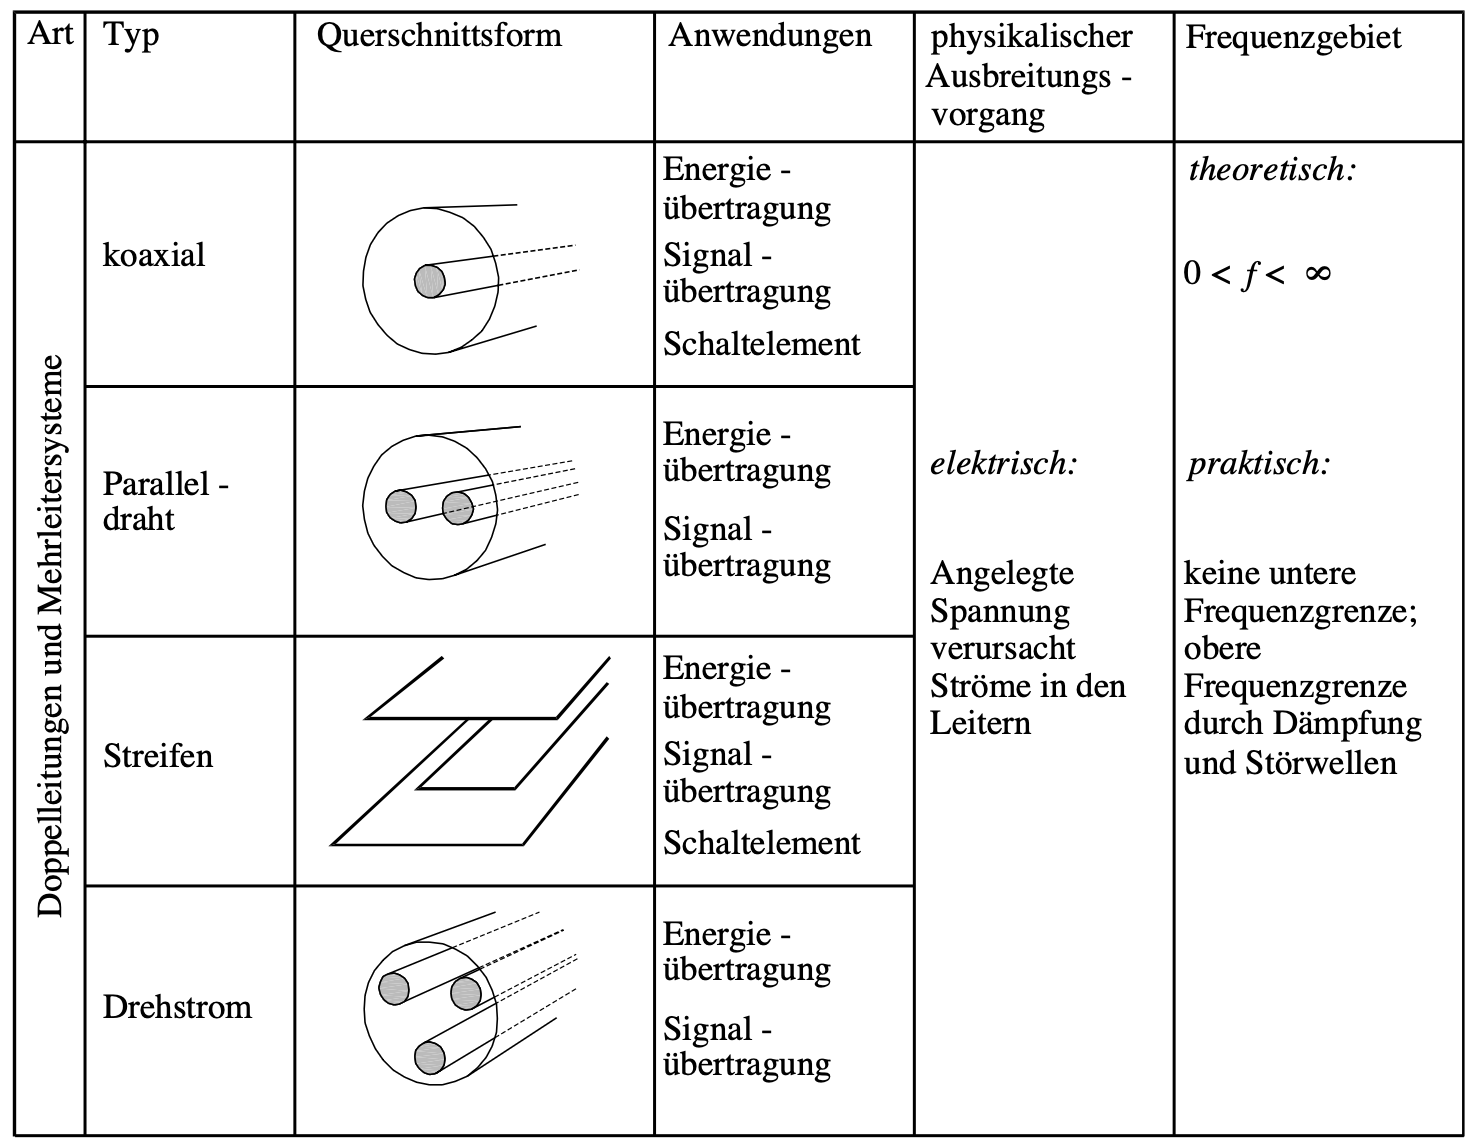
\includegraphics[width=0.75\textwidth]{../Ausarbeitung/images/Leiter.png}
    \end{center}
\end{figure}

\end{frame}


\begin{frame}{Leitungsbeläge}
Auf einem Leitungsstück der Länge $s$ mit Widerstand $R_{s}$ erzeugen elektrische und magnetische Felder
\begin{figure}[!htb]
    \begin{center}
        \includegraphics[width=0.5\textwidth]{graphics/Ersatzschaltbild1/document}
    \end{center}
\end{figure}
\begin{itemize}
    \item Induktion $L_{s}$
    \item Kapazität $C_{s}$ und
    \item Querleitwert $G_{s}$
\end{itemize}

\end{frame}


\begin{frame}{Leitungsbeläge}
Definiere Induktionsbelag $L^{\prime} = \frac{L_{s}}{s}$ als Längsinduktivität pro Längeneinheit.
Analog definieren wir
\begin{itemize}
    \item Kapazitätbelag $C^{\prime} = \frac{C_{s}}{s}$
    \item Leitwertsbelag $G^{\prime} = \frac{G_{s}}{s}$
    \item Widerstandsbelag $R^{\prime} = \frac{R_{s}}{s}$
\end{itemize}

\end{frame}


\begin{frame}{Spannung auf infinitesimalem Leitungsstück}
Wir stellen uns ein infinitesimales Leitungsstück der Länge $\mathrm{d}z$ vor:
\begin{figure}[!htb]
    \begin{center}
        \includegraphics[width=0.5\textwidth]{graphics/Ersatzschaltbild2/document}
    \end{center}
\end{figure}
Widerstand $R^{\prime} \, \mathrm{d}z$ und Induktivität $L^{\prime} \, \mathrm{d}z$ verursachen einen Spannungsabfall
von
\[
i \, R^{\prime} \, \mathrm{d}z + \frac{\partial i}{\partial t} \, L^{\prime} \, \mathrm{d}z.
\]
Mit der Kirchhoffschen Maschengleichung~\cite{Kirchhoff} folgt
\begin{equation*}
    u = i \, R^{\prime} \, \mathrm{d}z + \frac{\partial i}{\partial t} \, L^{\prime} \, \mathrm{d}z +
    \frac{\partial u}{\partial z} \mathrm{d}{z}.
\end{equation*}

\end{frame}


\begin{frame}{Strom auf infinitesimalem Leitungsstück}
Durch Querleitwert $G^{\prime} \, \mathrm{d}z$ und Querkapazität $C^{\prime} \, \mathrm{d}z$ fließt der Strom
\[
u \, G^{\prime} \, \mathrm{d}z + \frac{\partial u}{\partial t} \, C^{\prime} \, \mathrm{d}z.
\]
Mit der Kirchhoffschen Knotenregel~\cite{Kirchhoff} folgt
\begin{equation*}
    i = u \, G^{\prime} \, \mathrm{d}z + \frac{\partial u}{\partial t} \, C^{\prime} \, \mathrm{d}z + i +
    \frac{\partial i}{\partial z} \mathrm{d}z.
\end{equation*}

\end{frame}


\begin{frame}{Differentialgleichungen der elektrischen Leitung}
Durch teilen beider Gleichungen durch $\mathrm{d}z$ erhalten wir die \alert{Gleichungen des elektrischen Leiters}
\begin{align}
    \frac{\partial u}{\partial z} &= -\left(R^{\prime} + L^{\prime}\frac{\partial}{\partial t}\right)i \label{eq:Dgl1}
    \\[1ex]
    \frac{\partial i}{\partial z} &= -\left(G^{\prime} + C^{\prime}\frac{\partial}{\partial t}\right)u. \label{eq:Dgl2}
\end{align}
Äquivalent hierzu sind die \alert{Telegraphenleitungen}
\begin{align}
    \frac{\partial^{2} u}{\partial z^{2}} &= R^{\prime} G^{\prime} u(z,t) + (R^{\prime} C^{\prime} + L^{\prime}
    G^{\prime}) \frac{\partial u(z, t)}{\partial t} + L^{\prime} C^{\prime} \frac{\partial^{2} u(z,t)}{\partial t^{2}}
    \label{eq:Tele1} \\[1.5ex]
    \frac{\partial^{2} i}{\partial z^{2}} &= R^{\prime} G^{\prime} i(z,t) + (R^{\prime} C^{\prime} + L^{\prime}
    G^{\prime}) \frac{\partial i(z, t)}{\partial t} + L^{\prime} C^{\prime} \frac{\partial^{2} i(z, t)}{\partial t^{2}}.
\end{align}

\end{frame}


\section{Lösung der Telegraphenleitung}


\begin{frame}{Eingeschwungener Zustand}
Wir machen folgende Annahmen:
\begin{itemize}
    \item<1-> ignoriere Einschwungvorgang
    \item<2-> zeitlich sinusförmiger Verlauf
    \item<3-> nur eine Schwingung mit Kreisfrequenz $\omega$
\end{itemize}

\vspace*{1em}
\onslide<4->{
Dann lassen sich Strom und Spannung mittels sogenannter Phasoren $\underline{I}$ und $\underline{U}$ darstellen:
\begin{align}
    u(z, t) &= \mathrm{Re} \left[ \underline{U}(z) \exp(\mathrm{j} \omega t) \right] \label{eq:Spannung} \\
    i(z, t) &= \mathrm{Re} \left[ \underline{I}(z) \exp(\mathrm{j} \omega t) \right]
\end{align}
}

\end{frame}


\begin{frame}{Differentialgleichungssystem}
Wir erhalten
\begin{align}
    \frac{\text{d}^{2} \underline{U}}{\text{d} z^{2}} &= \gamma^{2} \underline{U} \label{eq:VerlustDgl1} \\[1ex]
    \frac{\text{d}^{2} \underline{I}}{\text{d} z^{2}} &= \gamma^{2} \underline{I} \label{eq:VerlustDgl2} \\[1ex]
    \gamma^{2} &= \left( R^{\prime} + \mathrm{j} \omega L^{\prime} \right) \left( G^{\prime} + \mathrm{j} \omega
    C^{\prime} \right) \label{eq:Gamma}.
\end{align}
Man nennt $\gamma$ die Wellenausbreitungsgeschwindigkeit.

\end{frame}


\begin{frame}{Verlustlose Leitung}
Verlustlosen Fall ist gegeben durch \mbox{$R^{\prime} = G^{\prime} = 0$}.

Die Gleichungen vereinfachen sich zu
\begin{align}
    \frac{\partial u}{\partial z} &= - L^{\prime} \, \frac{\partial i}{\partial t} \label{eq:Dgl7} \\[1ex]
    \frac{\partial i}{\partial z} &= - C^{\prime} \, \frac{\partial u}{\partial t} \label{eq:Dgl8} .
\end{align}
Dies sind jeweils Wellengleichungen, deren Lösung sich aus zwei Partiallösungen zusammensetzt,
\begin{align}
    u(z, t) &= u_{h}(v t - z) + u_{r}(v t + z) \label{eq:AllgEq1} \\[1ex]
    i(z, t) &= i_{h}(v t - z) + i_{r}(v t + z) \label{eq:AllgEq2}.
\end{align}
$v$ ist die Wellengeschwindigkeit.
Wir nennen $u_{h}$ \alert{vor-}, $u_{r}$ \alert{rücklaufende Welle}!
\end{frame}


\begin{frame}{Allgemeine Lösung}
    Lösungen haben die Form
    \begin{equation}
        \underline{U}(z) = \underline{U}_{1} \mathrm{e}^{- \gamma z}
        +
        \underline{U}_{2} \mathrm{e}^{\gamma z}
        = \underline{U}_{h} + \underline{U}_{r} \label{eq:VerlustU}
    \end{equation}
    und
    \begin{equation}
        \underline{I}(z) = \frac{1}{Z_{w}} \left( \vphantom{\sqrt{1}{Z}}
        \underline{U}_{1} \mathrm{e}^{- \gamma z} - \underline{U}_{2} \mathrm{e}^{\gamma z} \right)
        = \underline{I}_{h} + \underline{I}_{r}, \label{eq:VerlustI}
    \end{equation}
    wobei
    \begin{equation}
        Z_{w} = \sqrt{\frac{R^{\prime} + \mathrm{j} \omega L^{\prime}}{G^{\prime} + \mathrm{j} \omega C^{\prime}}}
        \label{eq:Zw}
    \end{equation}
    der Wellenwiderstand oder Wellenimpedanz genannt wird.

\end{frame}


\begin{frame}{Wellenwiderstand}
Es gilt
\begin{equation*}
    \frac{\underline{U}}{\underline{I}} =
     Z_{w} \frac{\underline{U}_{h} + \underline{U}_{r}}{\underline{I}_{h} + \underline{I}_{r}} \ne const.
\end{equation*}
entlang des Leiters, aber
\[ \frac{\underline{U}_{h}}{\underline{I}_{h}} = \frac{\underline{U}_{r}}{- \underline{I}_{r}} = Z_{w}! \]

\end{frame}



\begin{frame}{Randbedingungen}

\end{frame}




\begin{frame}{Literaturverzeichnis}
\printbibliography
\end{frame}

\end{document}
